% Options for packages loaded elsewhere
\PassOptionsToPackage{unicode}{hyperref}
\PassOptionsToPackage{hyphens}{url}
\PassOptionsToPackage{dvipsnames,svgnames,x11names}{xcolor}
%
\documentclass[
  letterpaper,
  DIV=11,
  numbers=noendperiod]{scrreprt}

\usepackage{amsmath,amssymb}
\usepackage{iftex}
\ifPDFTeX
  \usepackage[T1]{fontenc}
  \usepackage[utf8]{inputenc}
  \usepackage{textcomp} % provide euro and other symbols
\else % if luatex or xetex
  \usepackage{unicode-math}
  \defaultfontfeatures{Scale=MatchLowercase}
  \defaultfontfeatures[\rmfamily]{Ligatures=TeX,Scale=1}
\fi
\usepackage{lmodern}
\ifPDFTeX\else  
    % xetex/luatex font selection
\fi
% Use upquote if available, for straight quotes in verbatim environments
\IfFileExists{upquote.sty}{\usepackage{upquote}}{}
\IfFileExists{microtype.sty}{% use microtype if available
  \usepackage[]{microtype}
  \UseMicrotypeSet[protrusion]{basicmath} % disable protrusion for tt fonts
}{}
\makeatletter
\@ifundefined{KOMAClassName}{% if non-KOMA class
  \IfFileExists{parskip.sty}{%
    \usepackage{parskip}
  }{% else
    \setlength{\parindent}{0pt}
    \setlength{\parskip}{6pt plus 2pt minus 1pt}}
}{% if KOMA class
  \KOMAoptions{parskip=half}}
\makeatother
\usepackage{xcolor}
\setlength{\emergencystretch}{3em} % prevent overfull lines
\setcounter{secnumdepth}{5}
% Make \paragraph and \subparagraph free-standing
\ifx\paragraph\undefined\else
  \let\oldparagraph\paragraph
  \renewcommand{\paragraph}[1]{\oldparagraph{#1}\mbox{}}
\fi
\ifx\subparagraph\undefined\else
  \let\oldsubparagraph\subparagraph
  \renewcommand{\subparagraph}[1]{\oldsubparagraph{#1}\mbox{}}
\fi

\usepackage{color}
\usepackage{fancyvrb}
\newcommand{\VerbBar}{|}
\newcommand{\VERB}{\Verb[commandchars=\\\{\}]}
\DefineVerbatimEnvironment{Highlighting}{Verbatim}{commandchars=\\\{\}}
% Add ',fontsize=\small' for more characters per line
\usepackage{framed}
\definecolor{shadecolor}{RGB}{241,243,245}
\newenvironment{Shaded}{\begin{snugshade}}{\end{snugshade}}
\newcommand{\AlertTok}[1]{\textcolor[rgb]{0.68,0.00,0.00}{#1}}
\newcommand{\AnnotationTok}[1]{\textcolor[rgb]{0.37,0.37,0.37}{#1}}
\newcommand{\AttributeTok}[1]{\textcolor[rgb]{0.40,0.45,0.13}{#1}}
\newcommand{\BaseNTok}[1]{\textcolor[rgb]{0.68,0.00,0.00}{#1}}
\newcommand{\BuiltInTok}[1]{\textcolor[rgb]{0.00,0.23,0.31}{#1}}
\newcommand{\CharTok}[1]{\textcolor[rgb]{0.13,0.47,0.30}{#1}}
\newcommand{\CommentTok}[1]{\textcolor[rgb]{0.37,0.37,0.37}{#1}}
\newcommand{\CommentVarTok}[1]{\textcolor[rgb]{0.37,0.37,0.37}{\textit{#1}}}
\newcommand{\ConstantTok}[1]{\textcolor[rgb]{0.56,0.35,0.01}{#1}}
\newcommand{\ControlFlowTok}[1]{\textcolor[rgb]{0.00,0.23,0.31}{#1}}
\newcommand{\DataTypeTok}[1]{\textcolor[rgb]{0.68,0.00,0.00}{#1}}
\newcommand{\DecValTok}[1]{\textcolor[rgb]{0.68,0.00,0.00}{#1}}
\newcommand{\DocumentationTok}[1]{\textcolor[rgb]{0.37,0.37,0.37}{\textit{#1}}}
\newcommand{\ErrorTok}[1]{\textcolor[rgb]{0.68,0.00,0.00}{#1}}
\newcommand{\ExtensionTok}[1]{\textcolor[rgb]{0.00,0.23,0.31}{#1}}
\newcommand{\FloatTok}[1]{\textcolor[rgb]{0.68,0.00,0.00}{#1}}
\newcommand{\FunctionTok}[1]{\textcolor[rgb]{0.28,0.35,0.67}{#1}}
\newcommand{\ImportTok}[1]{\textcolor[rgb]{0.00,0.46,0.62}{#1}}
\newcommand{\InformationTok}[1]{\textcolor[rgb]{0.37,0.37,0.37}{#1}}
\newcommand{\KeywordTok}[1]{\textcolor[rgb]{0.00,0.23,0.31}{#1}}
\newcommand{\NormalTok}[1]{\textcolor[rgb]{0.00,0.23,0.31}{#1}}
\newcommand{\OperatorTok}[1]{\textcolor[rgb]{0.37,0.37,0.37}{#1}}
\newcommand{\OtherTok}[1]{\textcolor[rgb]{0.00,0.23,0.31}{#1}}
\newcommand{\PreprocessorTok}[1]{\textcolor[rgb]{0.68,0.00,0.00}{#1}}
\newcommand{\RegionMarkerTok}[1]{\textcolor[rgb]{0.00,0.23,0.31}{#1}}
\newcommand{\SpecialCharTok}[1]{\textcolor[rgb]{0.37,0.37,0.37}{#1}}
\newcommand{\SpecialStringTok}[1]{\textcolor[rgb]{0.13,0.47,0.30}{#1}}
\newcommand{\StringTok}[1]{\textcolor[rgb]{0.13,0.47,0.30}{#1}}
\newcommand{\VariableTok}[1]{\textcolor[rgb]{0.07,0.07,0.07}{#1}}
\newcommand{\VerbatimStringTok}[1]{\textcolor[rgb]{0.13,0.47,0.30}{#1}}
\newcommand{\WarningTok}[1]{\textcolor[rgb]{0.37,0.37,0.37}{\textit{#1}}}

\providecommand{\tightlist}{%
  \setlength{\itemsep}{0pt}\setlength{\parskip}{0pt}}\usepackage{longtable,booktabs,array}
\usepackage{calc} % for calculating minipage widths
% Correct order of tables after \paragraph or \subparagraph
\usepackage{etoolbox}
\makeatletter
\patchcmd\longtable{\par}{\if@noskipsec\mbox{}\fi\par}{}{}
\makeatother
% Allow footnotes in longtable head/foot
\IfFileExists{footnotehyper.sty}{\usepackage{footnotehyper}}{\usepackage{footnote}}
\makesavenoteenv{longtable}
\usepackage{graphicx}
\makeatletter
\def\maxwidth{\ifdim\Gin@nat@width>\linewidth\linewidth\else\Gin@nat@width\fi}
\def\maxheight{\ifdim\Gin@nat@height>\textheight\textheight\else\Gin@nat@height\fi}
\makeatother
% Scale images if necessary, so that they will not overflow the page
% margins by default, and it is still possible to overwrite the defaults
% using explicit options in \includegraphics[width, height, ...]{}
\setkeys{Gin}{width=\maxwidth,height=\maxheight,keepaspectratio}
% Set default figure placement to htbp
\makeatletter
\def\fps@figure{htbp}
\makeatother
\newlength{\cslhangindent}
\setlength{\cslhangindent}{1.5em}
\newlength{\csllabelwidth}
\setlength{\csllabelwidth}{3em}
\newlength{\cslentryspacingunit} % times entry-spacing
\setlength{\cslentryspacingunit}{\parskip}
\newenvironment{CSLReferences}[2] % #1 hanging-ident, #2 entry spacing
 {% don't indent paragraphs
  \setlength{\parindent}{0pt}
  % turn on hanging indent if param 1 is 1
  \ifodd #1
  \let\oldpar\par
  \def\par{\hangindent=\cslhangindent\oldpar}
  \fi
  % set entry spacing
  \setlength{\parskip}{#2\cslentryspacingunit}
 }%
 {}
\usepackage{calc}
\newcommand{\CSLBlock}[1]{#1\hfill\break}
\newcommand{\CSLLeftMargin}[1]{\parbox[t]{\csllabelwidth}{#1}}
\newcommand{\CSLRightInline}[1]{\parbox[t]{\linewidth - \csllabelwidth}{#1}\break}
\newcommand{\CSLIndent}[1]{\hspace{\cslhangindent}#1}

\KOMAoption{captions}{tableheading}
\makeatletter
\@ifpackageloaded{tcolorbox}{}{\usepackage[skins,breakable]{tcolorbox}}
\@ifpackageloaded{fontawesome5}{}{\usepackage{fontawesome5}}
\definecolor{quarto-callout-color}{HTML}{909090}
\definecolor{quarto-callout-note-color}{HTML}{0758E5}
\definecolor{quarto-callout-important-color}{HTML}{CC1914}
\definecolor{quarto-callout-warning-color}{HTML}{EB9113}
\definecolor{quarto-callout-tip-color}{HTML}{00A047}
\definecolor{quarto-callout-caution-color}{HTML}{FC5300}
\definecolor{quarto-callout-color-frame}{HTML}{acacac}
\definecolor{quarto-callout-note-color-frame}{HTML}{4582ec}
\definecolor{quarto-callout-important-color-frame}{HTML}{d9534f}
\definecolor{quarto-callout-warning-color-frame}{HTML}{f0ad4e}
\definecolor{quarto-callout-tip-color-frame}{HTML}{02b875}
\definecolor{quarto-callout-caution-color-frame}{HTML}{fd7e14}
\makeatother
\makeatletter
\makeatother
\makeatletter
\@ifpackageloaded{bookmark}{}{\usepackage{bookmark}}
\makeatother
\makeatletter
\@ifpackageloaded{caption}{}{\usepackage{caption}}
\AtBeginDocument{%
\ifdefined\contentsname
  \renewcommand*\contentsname{Table of contents}
\else
  \newcommand\contentsname{Table of contents}
\fi
\ifdefined\listfigurename
  \renewcommand*\listfigurename{List of Figures}
\else
  \newcommand\listfigurename{List of Figures}
\fi
\ifdefined\listtablename
  \renewcommand*\listtablename{List of Tables}
\else
  \newcommand\listtablename{List of Tables}
\fi
\ifdefined\figurename
  \renewcommand*\figurename{Figure}
\else
  \newcommand\figurename{Figure}
\fi
\ifdefined\tablename
  \renewcommand*\tablename{Table}
\else
  \newcommand\tablename{Table}
\fi
}
\@ifpackageloaded{float}{}{\usepackage{float}}
\floatstyle{ruled}
\@ifundefined{c@chapter}{\newfloat{codelisting}{h}{lop}}{\newfloat{codelisting}{h}{lop}[chapter]}
\floatname{codelisting}{Listing}
\newcommand*\listoflistings{\listof{codelisting}{List of Listings}}
\makeatother
\makeatletter
\@ifpackageloaded{caption}{}{\usepackage{caption}}
\@ifpackageloaded{subcaption}{}{\usepackage{subcaption}}
\makeatother
\makeatletter
\@ifpackageloaded{tcolorbox}{}{\usepackage[skins,breakable]{tcolorbox}}
\makeatother
\makeatletter
\@ifundefined{shadecolor}{\definecolor{shadecolor}{rgb}{.97, .97, .97}}
\makeatother
\makeatletter
\makeatother
\makeatletter
\makeatother
\ifLuaTeX
  \usepackage{selnolig}  % disable illegal ligatures
\fi
\IfFileExists{bookmark.sty}{\usepackage{bookmark}}{\usepackage{hyperref}}
\IfFileExists{xurl.sty}{\usepackage{xurl}}{} % add URL line breaks if available
\urlstyle{same} % disable monospaced font for URLs
\hypersetup{
  pdftitle={Getting Started with R},
  pdfauthor={Zachary M. Smith},
  colorlinks=true,
  linkcolor={blue},
  filecolor={Maroon},
  citecolor={Blue},
  urlcolor={Blue},
  pdfcreator={LaTeX via pandoc}}

\title{Getting Started with R}
\author{Zachary M. Smith}
\date{2023-09-07}

\begin{document}
\maketitle
\ifdefined\Shaded\renewenvironment{Shaded}{\begin{tcolorbox}[frame hidden, breakable, borderline west={3pt}{0pt}{shadecolor}, interior hidden, enhanced, sharp corners, boxrule=0pt]}{\end{tcolorbox}}\fi

\renewcommand*\contentsname{Table of contents}
{
\hypersetup{linkcolor=}
\setcounter{tocdepth}{2}
\tableofcontents
}
\bookmarksetup{startatroot}

\hypertarget{preface}{%
\chapter*{Preface}\label{preface}}
\addcontentsline{toc}{chapter}{Preface}

\markboth{Preface}{Preface}

This book is intended to provide standard guidance for getting started
with R.

\bookmarksetup{startatroot}

\hypertarget{r-intro}{%
\chapter{R Intro}\label{r-intro}}

\hypertarget{what-is-r}{%
\section{What is R?}\label{what-is-r}}

R is an open source programming language developed for statistical
computing and graphic production. ``R can be considered as a different
implementation of S'', a language that was developed at Bell
Laboratories (https://www.r-project.org/about.html).

\hypertarget{benefits-of-using-r}{%
\subsection{Benefits of Using R}\label{benefits-of-using-r}}

\begin{enumerate}
\def\labelenumi{\arabic{enumi}.}
\tightlist
\item
  \textbf{Reproducibility:} Standardized processes (e.g., functions,
  loops, documentation)
\end{enumerate}

\begin{itemize}
\tightlist
\item
  When using MS Excel processes are often spread across multiple sheets
  or calculations are performed haphazardly within a single sheet. In
  general, this makes it very hard to interpret processes performed and
  to reproduce the process.
\end{itemize}

\begin{enumerate}
\def\labelenumi{\arabic{enumi}.}
\setcounter{enumi}{1}
\tightlist
\item
  \textbf{Power:} Ability to perform simple and complex data
  manipulations, iterative processes, and calculations
\end{enumerate}

\begin{itemize}
\item
  Access to more than 10,000 packages on CRAN
\item
  New packages are constantly being developed
\item
  New features are constantly being added to existing packages
\end{itemize}

\hypertarget{r-packages}{%
\subsection{R Packages}\label{r-packages}}

R packages are extensions of base R that provide additional features or
provide alternative functionality.

\begin{itemize}
\item
  Availability
\item
  CRAN (https://cran.r-project.org/)
\item
  The Comprehensive R Archive Network (CRAN)
\item
  FTP and web servers that store R Packages
\item
  Packages are required to meet certain standards
\item
  GitHub (https://github.com)
\item
  These packages are usually under development
\item
  Contains development versions of many packages available on CRAN
\item
  Custom (http://r-pkgs.had.co.nz/)
\item
  You have the ability to create your own packages.
\end{itemize}

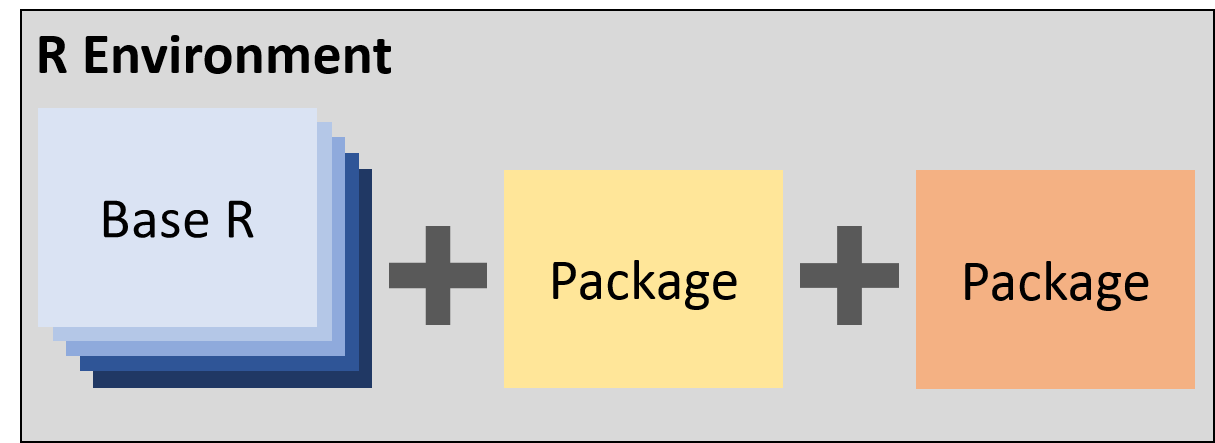
\includegraphics[width=7.29167in,height=\textheight]{images/introduction/packages.png}

\hypertarget{what-is-rstudio}{%
\section{What is RStudio?}\label{what-is-rstudio}}

\begin{tcolorbox}[enhanced jigsaw, title=\textcolor{quarto-callout-note-color}{\faInfo}\hspace{0.5em}{Note}, opacitybacktitle=0.6, left=2mm, colbacktitle=quarto-callout-note-color!10!white, opacityback=0, colframe=quarto-callout-note-color-frame, bottomrule=.15mm, coltitle=black, titlerule=0mm, toptitle=1mm, bottomtitle=1mm, breakable, arc=.35mm, colback=white, rightrule=.15mm, toprule=.15mm, leftrule=.75mm]

\texttt{RStudio\ !=\ R}

\end{tcolorbox}

RStudio is not R. RStudio is an Integrated Development Environment (IDE)
that makes it easier to develop with R. The desktop version of RStudio
is maintained by the company Posit and is free to download.

Another popular IDE is
\href{https://www.bing.com/search?q=vscode\&cvid=5af1606bae8d427391a6c59b8be84329\&aqs=edge.0.0l9j69i11004.3351j0j9\&FORM=ANAB01\&PC=U531}{Visual
Studio Code or VS Code} now owned by Microsoft.

\bookmarksetup{startatroot}

\hypertarget{quick-reference}{%
\chapter{Quick Reference}\label{quick-reference}}

Below are a collection of R related resources. If you have
recommendation you would like to see added to the list, please open a
pull request or issue via GitHub.

\begin{enumerate}
\def\labelenumi{\arabic{enumi}.}
\item
  \href{https://www.rstudio.com/resources/cheatsheets/}{Cheat Sheets}
\item
  \href{https://www.r-bloggers.com/}{R Bloggers}
\item
  Questions

  \begin{itemize}
  \item
    \href{https://stackoverflow.com}{StackOverflow}
  \item
    \href{https://community.rstudio.com/}{Posit Community}
  \end{itemize}
\item
  Style Guides

  \begin{itemize}
  \item
    \href{http://style.tidyverse.org/index.html}{Tidyverse Style Guide}
  \item
    \href{https://google.github.io/styleguide/Rguide.xml}{Google's Style
    Guide}
  \end{itemize}
\item
  Books and Papers

  \begin{itemize}
  \item
    \href{https://r4ds.hadley.nz/}{R for Data Science (2e)}
  \item
    \href{http://heather.cs.ucdavis.edu/~matloff/132/NSPpart.pdf}{The
    Art of R Programming}
  \item
    \href{http://adv-r.had.co.nz/}{Advanced R}
  \item
    \href{http://r-pkgs.had.co.nz/}{R Packages}
  \item
    \href{https://www.jstatsoft.org/article/view/v059i10}{Tidy Data}
  \end{itemize}
\item
  Packages

  \begin{itemize}
  \item
    \href{https://shiny.rstudio.com/}{Shiny (Interactive Apps)}

    \begin{itemize}
    \tightlist
    \item
      \href{https://shiny.rstudio.com/tutorial/}{Tutorials}
    \end{itemize}
  \item
    \href{https://rstudio.github.io/leaflet/}{Leaflet (Interactive
    Maps)}
  \item
    \href{https://rstudio.github.io/DT/}{DT (Interactive Tables)}
  \item
    \href{https://rstudio.github.io/dygraphs/}{Dygraphs (Interactive
    Time Series Plots)}
  \item
    \href{https://plot.ly/r/}{Plotly (Interactive Plots)}
  \item
    \href{https://www.tidyverse.org/}{Tidyverse Packages (Ecosystem of
    Packages)}
  \item
    \href{https://rmarkdown.rstudio.com/lesson-1.html}{Rmarkdown
    (Documentation)}
  \item
    \href{https://github.com/USGS-R}{USGS GitHub}

    \begin{itemize}
    \item
      \href{https://cran.r-project.org/web/packages/dataRetrieval/vignettes/dataRetrieval.html}{dataRetrieval
      (Acquire data from the Water Quality Portal)}
    \item
      \href{https://cran.r-project.org/web/packages/EGRET/vignettes/EGRET.pdf}{EGRET
      (Analysis of long-term changes in water quality and streamflow)}
    \end{itemize}
  \end{itemize}
\end{enumerate}

\bookmarksetup{startatroot}

\hypertarget{installation}{%
\chapter{Installation}\label{installation}}

Use the following links to install R and RStudio by following the links
below. I highly recommend that you also install Git (link below) and
create an account on GitHub (link below). The Git related tools are very
useful but

\begin{longtable}[]{@{}
  >{\raggedright\arraybackslash}p{(\columnwidth - 2\tabcolsep) * \real{0.1304}}
  >{\raggedright\arraybackslash}p{(\columnwidth - 2\tabcolsep) * \real{0.8696}}@{}}
\toprule\noalign{}
\begin{minipage}[b]{\linewidth}\raggedright
Software
\end{minipage} & \begin{minipage}[b]{\linewidth}\raggedright
Link
\end{minipage} \\
\midrule\noalign{}
\endhead
\bottomrule\noalign{}
\endlastfoot
R & \url{https://cran.r-project.org/bin/windows/base/} \\
RStudio &
\url{https://www.rstudio.com/products/rstudio/download/\#download} \\
Git & \url{https://git-scm.com/downloads} \\
GitHub & \url{https://github.com} \\
\end{longtable}

\bookmarksetup{startatroot}

\hypertarget{updating-software-and-packages}{%
\chapter{Updating Software and
Packages}\label{updating-software-and-packages}}

\hypertarget{r}{%
\subsection{R}\label{r}}

Run the following code in the RGui, \textbf{NOT} in RStudio. The RGui
should be installed when you install R. On my Windows machine, I access
R by clicking on the R program file, ``R x64 3.5.1''.

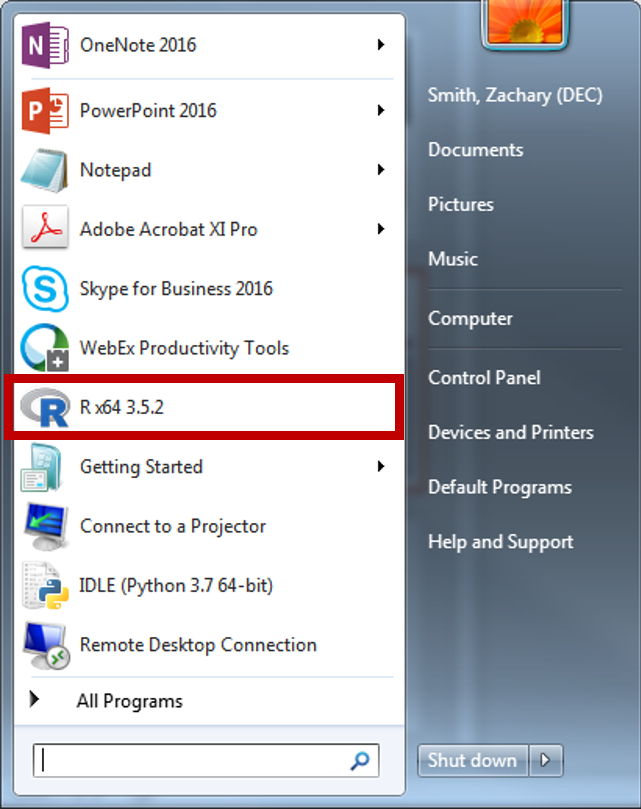
\includegraphics[width=4.16667in,height=\textheight]{images/installation_updates/rgui_program.png}

You should get a window like this if you have opened the correct
program.

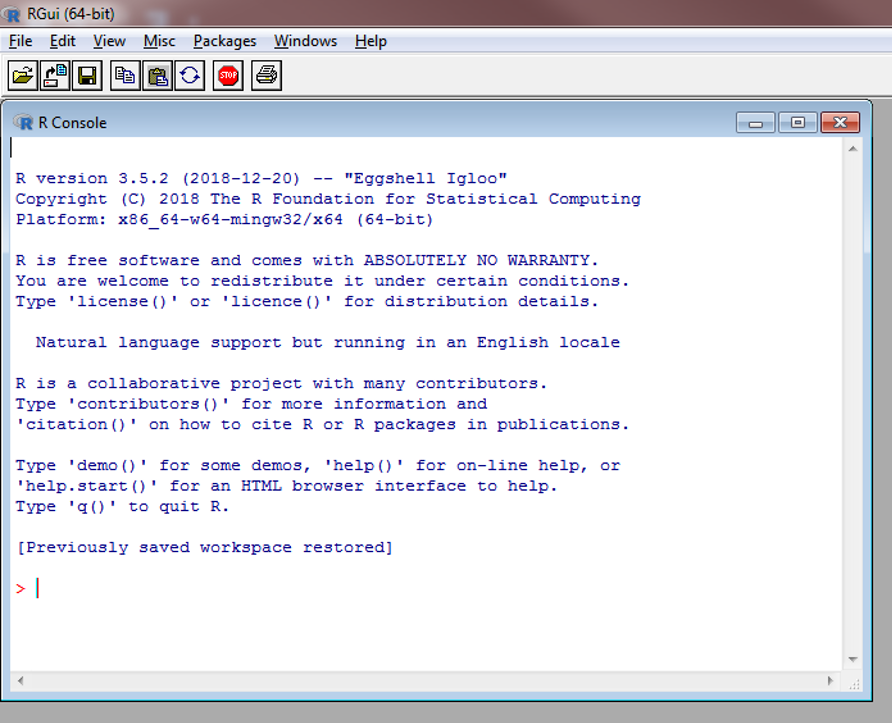
\includegraphics[width=4.16667in,height=\textheight]{images/installation_updates/rgui.png}

This code was copied from:
https://www.r-statistics.com/2013/03/updating-r-from-r-on-windows-using-the-installr-package/).
Make sure R Studio is closed before running this code within the RGui.

\begin{Shaded}
\begin{Highlighting}[]
\CommentTok{\# installing/loading the package:}

\ControlFlowTok{if}\NormalTok{(}\SpecialCharTok{!}\FunctionTok{require}\NormalTok{(installr)) \{}

\FunctionTok{install.packages}\NormalTok{(}\StringTok{"installr"}\NormalTok{);}

\FunctionTok{require}\NormalTok{(installr)}

\NormalTok{\} }\CommentTok{\#load / install+load installr}

\CommentTok{\# using the package:}

\FunctionTok{updateR}\NormalTok{()}
\end{Highlighting}
\end{Shaded}

\hypertarget{rstudio}{%
\subsection{RStudio}\label{rstudio}}

\begin{enumerate}
\def\labelenumi{\arabic{enumi}.}
\item
  Open RStudio
\item
  Click on ``Help'' on the toolbar
\item
  Click on ``Check for Updates''
\item
  Follow instructions
\end{enumerate}

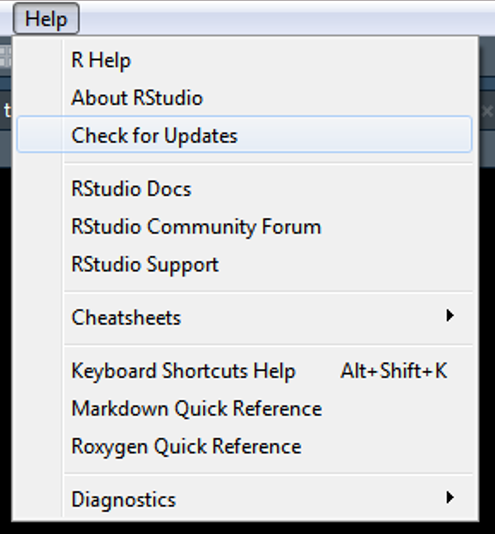
\includegraphics[width=4.16667in,height=\textheight]{images/installation_updates/update_rstudio.png}

\hypertarget{r-packages-1}{%
\subsection{R-Packages}\label{r-packages-1}}

\begin{enumerate}
\def\labelenumi{\arabic{enumi}.}
\item
  Open RStudio
\item
  Click on ``Tools'' on the toolbar
\item
  Click on ``Check for Package Updates\ldots{}''
\item
  Follow instructions
\end{enumerate}

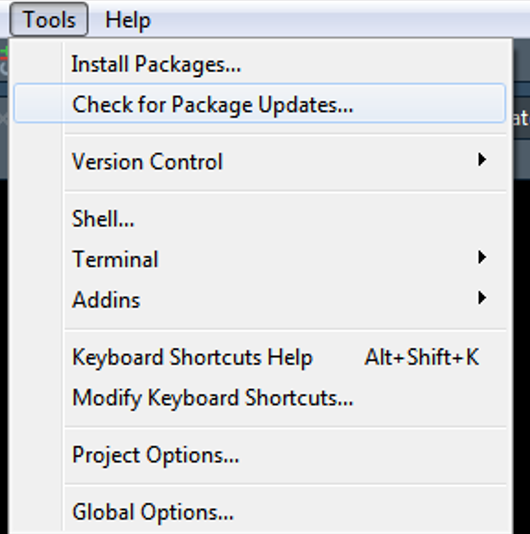
\includegraphics[width=4.16667in,height=\textheight]{images/installation_updates/update_packages.png}

\hypertarget{packages-for-workshop}{%
\subsubsection{Packages for Workshop}\label{packages-for-workshop}}

Please run the following code within RStudio to make sure you have all
of necessary packages for this workshop installed.

\begin{enumerate}
\def\labelenumi{\arabic{enumi}.}
\item
  Open RStudio
\item
  Copy the following code
\end{enumerate}

\begin{Shaded}
\begin{Highlighting}[]
\NormalTok{package.vec }\OtherTok{\textless{}{-}} \FunctionTok{c}\NormalTok{(}\StringTok{"tidyverse"}\NormalTok{, }\StringTok{"lubridate"}\NormalTok{,}

\StringTok{"knitr"}\NormalTok{, }\StringTok{"rmarkdown"}\NormalTok{, }\StringTok{"markdown"}\NormalTok{, }\StringTok{"caTools"}\NormalTok{, }\StringTok{"bitops"}\NormalTok{,}

\StringTok{"DT"}\NormalTok{, }\StringTok{"leaflet"}\NormalTok{, }\StringTok{"shiny"}\NormalTok{, }\StringTok{"jsonlite"}\NormalTok{,}

\StringTok{"data.table"}\NormalTok{, }\StringTok{"rprojroot"}\NormalTok{, }\StringTok{"viridis"}\NormalTok{)}

\FunctionTok{install.packages}\NormalTok{(package.vec)}
\end{Highlighting}
\end{Shaded}

\begin{enumerate}
\def\labelenumi{\arabic{enumi}.}
\setcounter{enumi}{2}
\tightlist
\item
  Paste the code into the Console within RStudio
\end{enumerate}

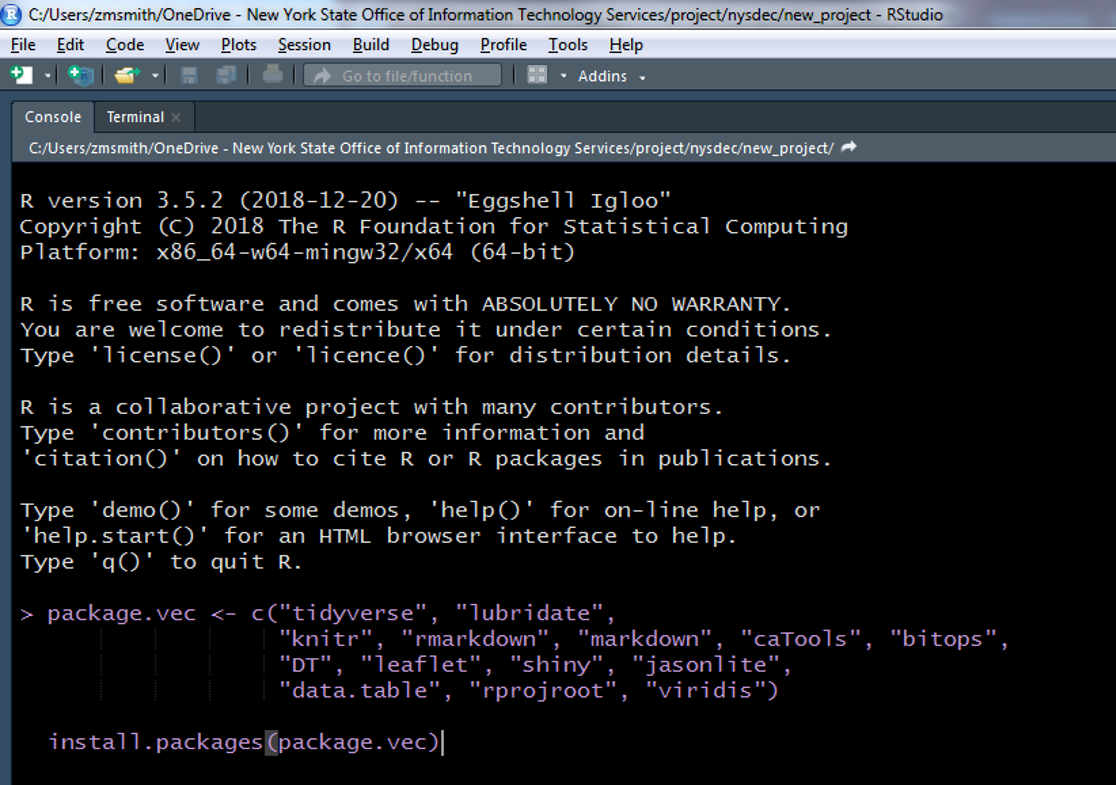
\includegraphics[width=4.16667in,height=\textheight]{images/installation_updates/install_packages.png}

\begin{enumerate}
\def\labelenumi{\arabic{enumi}.}
\setcounter{enumi}{3}
\tightlist
\item
  Hit Enter
\end{enumerate}

\begin{itemize}
\item
  If prompted with ``Do you want to restart R prior to installing?'',
  select ``Yes''
\item
  If prompted again then select ``No''
\end{itemize}

\begin{enumerate}
\def\labelenumi{\arabic{enumi}.}
\setcounter{enumi}{4}
\tightlist
\item
  The packages should begin to install. This may take some time.
\end{enumerate}

\bookmarksetup{startatroot}

\hypertarget{references}{%
\chapter*{References}\label{references}}
\addcontentsline{toc}{chapter}{References}

\markboth{References}{References}

\hypertarget{refs}{}
\begin{CSLReferences}{0}{0}
\end{CSLReferences}



\end{document}
